% !TeX root = ../main.tex
\chapter{检测平台搭建与调试}\label{ch:impl}

本章将具体实现上一章中设计的检测平台,
%TODO:intro



\section{电路实现与调试}\label{sec:impl-pcb}

本节讨论\ref{sec:rig-ctrl}节电控系统中所有自行设计的电子模块的具体实现,主要包括万用板、PCB的设计与制作,电路的调试以及性能测试等。


\subsection{背吹控制系统接口}\label{sec:impl-pcb-pressure}

由于背吹控制系统中的元件(压强变送器、电子比例阀、电磁方向阀)在试验台中较为接近(均可布置在底部),且均需要较高电压的直流电源(\SI{+24}{\V}与\SI{+12}{\V}),可将这三部分的接口电路集成在同一块PCB上。总体设计如图~\ref{fig:impl-pcb-pressure-sch-overall}:\SI{+24}{\V}单电源供电,通过稳压电路(``power'')获得其他所需电压;其他部分(\SIrange{4}{20}{\mA}电流环接口等)原理见\ref{sec:rig-ctrl}节。共使用4个标准可插拔式接线端子:\bverb|P1|接电源输入、\bverb|P2|接电流环、\bverb|P4|接电磁方向阀、\bverb|P5|接电子比例阀。\bverb|P5|接MCU(数据、数字供电),选用标准10针简单牛角接头。

稳压电路拓扑结构如图~\ref{fig:impl-pcb-pressure-sch-power}:\SI{+24}{\V}电源输入首先通过电源滤波保护电路(``line filter''),然后依次经过两级线性稳压芯片得到\SI{+12}{\V}与\SI{+5}{\V};同时,\SI{+12}{\V}还向精密\SI{+5}{\V}电压基准芯片供电,以提供ADC所需要的参考电压。滤波保护电路原理如图~\ref{fig:impl-pcb-pressure-sch-power-filter}:\bverb|D1|为防反接二极管;\bverb|L1|、\bverb|L2|为磁珠,对高频信号呈阻性,用于衰减高频电源噪声;\bverb|T1|为共模电感,与\bverb|C2|、\bverb|C3|、\bverb|C4|形成LC滤波器,用于消除电源纹波;\bverb|D2|为TVS(瞬态电压抑制)二极管,可防止电压尖峰损坏电路。这样既可对整个PCB乃至外部元件起到保护作用,又可降低模拟电路中因电源纹波产生的噪声。需要注意的是,虽然设计了板载滤波电路,仍不应直接使用开关电源供电,最好先经过外置直流电源滤波器消除较高能量的纹波,再接入PCB。

上述设计为v0.3.1版本,之前设计的v0.2.1版中不含板载电源滤波器,且其中第一级稳压电路为DC-DC开关转换器,实测发现模拟信号噪声极大,其中含有周期性的纹波成分以及频繁的尖峰,如\ref{fig:impl-pcb-pressure-emi-before};加入滤波电路后,各种噪声均显著降低,如\ref{fig:impl-pcb-pressure-emi-after}。

\begin{figure}[tbhp]
\centering
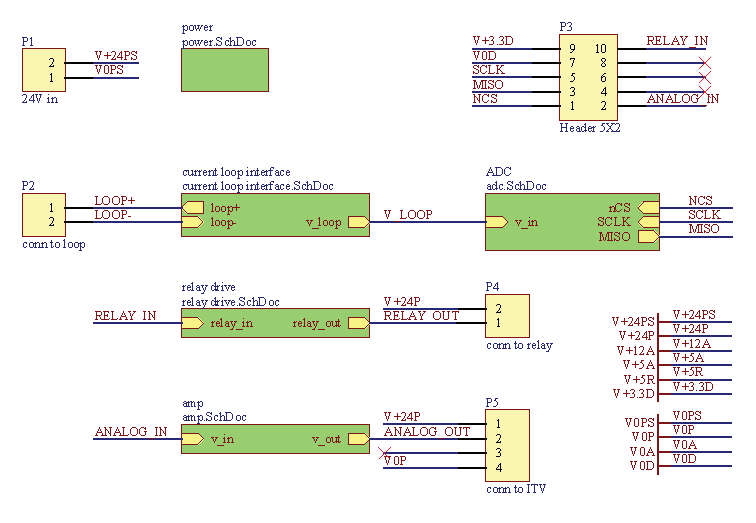
\includegraphics[width=1\linewidth]{impl/pcb__pressure__sch__overall}
\caption{背吹控制系统接口 -- 原理图 -- 总体}
\label{fig:impl-pcb-pressure-sch-overall}
\end{figure}

\begin{figure}[tbhp]
\centering
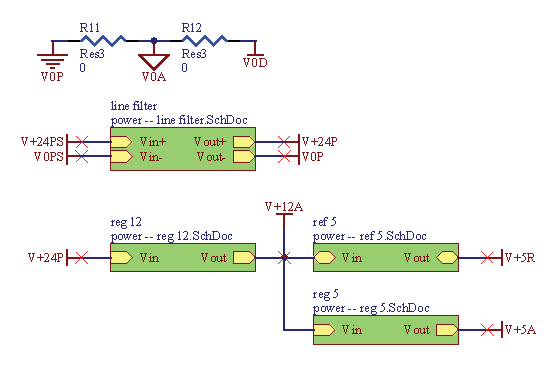
\includegraphics[width=0.75\linewidth]{impl/pcb__pressure__sch__power}
\caption{背吹控制系统接口 -- 原理图 -- 稳压}
\label{fig:impl-pcb-pressure-sch-power}
\end{figure}

\begin{figure}[p]
\centering
\includegraphics[width=0.9\linewidth]{impl/pcb__pressure__sch__power__filter}
\caption{背吹控制系统接口 -- 原理图 -- 滤波}
\label{fig:impl-pcb-pressure-sch-power-filter}
\end{figure}

\begin{figure}[p]
  \centering
  \begin{subfigure}{1\textwidth}
    \centering
    \includegraphics[height=0.33\textheight]{impl/pcb__pressure__emi__before.jpg}
    \caption{v0.2.1 无电源滤波}
    \label{fig:impl-pcb-pressure-emi-before}
  \end{subfigure}
  \begin{subfigure}{1\textwidth}
    \centering
    \includegraphics[height=0.33\textheight]{impl/pcb__pressure__emi__after.jpg}
    \caption{v0.3.1 有电源滤波}
    \label{fig:impl-pcb-pressure-emi-after}
  \end{subfigure}
\caption{背吹控制系统接口 -- 噪声}
\label{fig:impl-pcb-pressure-emi}
\end{figure}


\clearpage


\subsection{微力传感器接口}\label{sec:impl-pcb-ad7730}

\ref{sec:rig-ctrl-intf-strain}节中以AD7730为核心设计了微力传感器接口电路,本节将其实现为独立的PCB。根据图~\ref{fig:rig-ctrl-ad7730-ac}绘制完整的电路原理图(图~\ref{fig:impl-pcb-ad7730-sch})。电桥的激励端\bverb|E+|、\bverb|E-|与AD7730的参考输入接在一起,并可通过\bverb|J1|、\bverb|J2|跳线选择使用直流或交流激励:跳线2、3脚短接时,\bverb|E+|、\bverb|E-|分别接\SI{+5}{\V}与\SI{0}{\V},为直流激励;跳线1、2脚短接,并配置AD7730为交流激励模式后,AD7730输出\bverb|ACX|换向信号至DRV8837集成H桥芯片,向电桥施加交流激励,AD7730可自动处理正、反相信号,并补偿信号传输与开关延迟。\bverb|P1|接微力传感器(电桥),选用标准可插拔式接线端子;\bverb|P2|接MCU(数据、供电),选用标准10针简单牛角接头。

在制作PCB前,先在万用板上使用直插封装的AD7730制作了直流激励部分的电路,并使用已有的电桥传感器,接入MCU进行原理验证测试,确认了其功能一切正常;然后将LSB200微力传感器接入万用板进行测试,如图~\ref{fig:impl-pcb-ad7730-photo-perf},功能一切正常;最后,制作并焊接PCB,如图~\ref{fig:impl-pcb-ad7730-photo-pcb},实测总有效分辨率(包含传感器自身噪声在内)约为\SI{14}{\bit},完全满足性能要求。

\begin{figure}[tbhp]
\centering
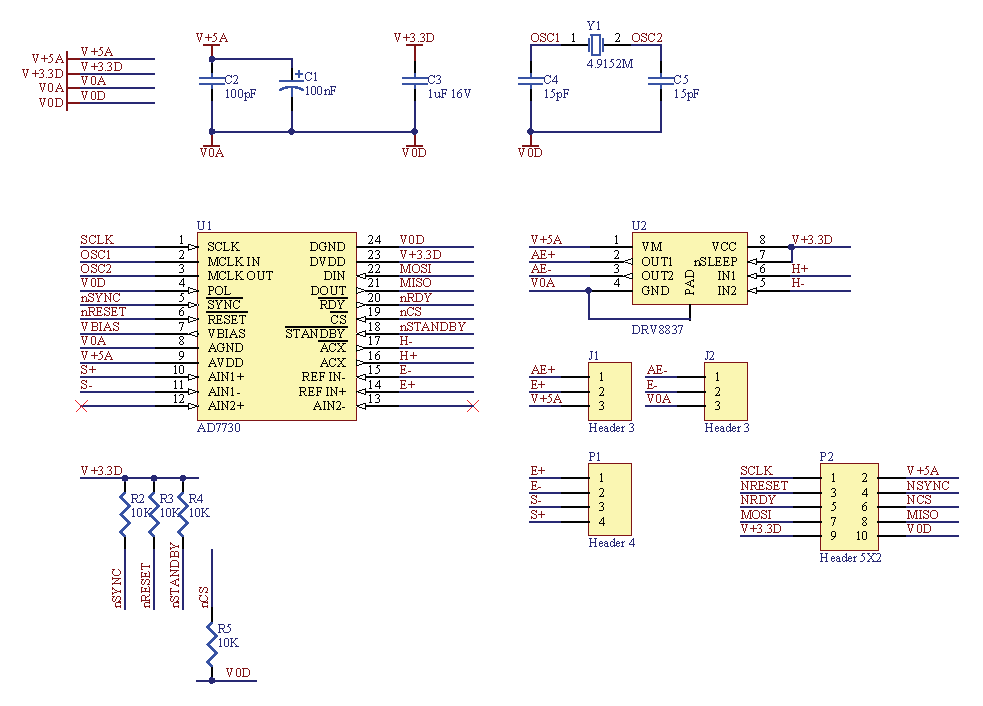
\includegraphics[width=1\linewidth]{impl/pcb__ad7730__sch}
\caption{AD7730电桥接口 -- 原理图}
\label{fig:impl-pcb-ad7730-sch}
\end{figure}

\begin{figure}[tbhp]
\centering
\includegraphics[width=0.8\linewidth]{impl/pcb__ad7730__photo__perf.jpg}
\caption{AD7730电桥接口 -- 万用板}
\label{fig:impl-pcb-ad7730-photo-perf}
\end{figure}

\begin{figure}[tbhp]
\centering
\includegraphics[width=0.4\linewidth]{impl/pcb__ad7730__photo__pcb.jpg}
\caption{AD7730电桥接口 -- PCB}
\label{fig:impl-pcb-ad7730-photo-pcb}
\end{figure}


\clearpage


\subsection{电动推杆零位传感器及接口}\label{sec:impl-pcb-zaber}

\ref{sec:rig-ctrl-intf-stepper}节为LAC-10A零位传感器设计了光耦隔离接口电路(图~\ref{fig:rig-ctrl-intf-opto}),由于其组成简单,直接用万用板与直插封装光耦制作,如图~\ref{fig:impl-pcb-zaber-opto-perf}:白色IC为光耦,色环电阻为光耦输入端限流电阻,右侧棕色的线表示直接焊在万用板上的贴片上拉电阻。

虽然使用该电路可减小误触发概率,但实测发现一个问题:当步进电机运行时,由于LAC-10A的零位传感器信号线与其步进电机接线处于同一电缆中,且无任何屏蔽措施,仅在步进电机处于上电保持状态时,其输出上的电磁干扰峰峰值($V_{\mathrm{pp}}$)就已超过\SI{8}{\V}(图~\ref{fig:impl-pcb-zaber-emi-before}),即使使用较高电压供电,也不能完全排除误触发现象。因此,为LAC-10A重新设计零位传感器,如图~\ref{fig:impl-pcb-zaber-new-sch}:采用同图~\ref{fig:impl-pcb-pressure-sch-power-filter}~类似的简易保护与滤波电路,并在传感器输出端加入滤波电容,以改善其抗干扰能力。由于需匹配电动推杆后部的安装尺寸,将该电路实现为PCB,安装后如图~\ref{fig:impl-pcb-zaber-new-photo}。上电实测发现电磁干扰得到有效控制,无误触发现象,与光耦接口电路配合可得到高质量的零位信号。

\begin{figure}[tbhp]
\centering
\includegraphics[width=0.618\linewidth]{impl/pcb__zaber__opto__perf.png}
\caption{LAC-10A零位传感器 -- 光耦接口 -- 万用板}
\label{fig:impl-pcb-zaber-opto-perf}
\end{figure}

\begin{figure}[tbhp]
\centering
\includegraphics[height=0.3\textheight]{impl/pcb__zaber__emi__before.jpg}
\caption{LAC-10A零位传感器 -- 电磁干扰}
\label{fig:impl-pcb-zaber-emi-before}
\end{figure}

\begin{figure}[p]
\centering
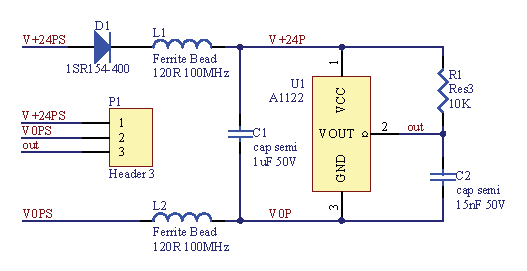
\includegraphics[width=0.75\linewidth]{impl/pcb__zaber__new__sch}
\caption{LAC-10A零位传感器 -- 新设计 -- 原理图}
\label{fig:impl-pcb-zaber-new-sch}
\end{figure}

\begin{figure}[p]
\centering
\includegraphics[height=0.3\textheight]{impl/pcb__zaber__new__photo.jpg}
\caption{LAC-10A零位传感器 -- 新设计 -- 实物图}
\label{fig:impl-pcb-zaber-new-photo}
\end{figure}





%-------------------------------------------------------
%                       stash
%-------------------------------------------------------



\clearpage



\section{stash}

由于LSB200微力传感器安全过载仅\SI{1}{\newton},装配时应特别小心,避免对其造成不可恢复的损伤。正确的装配方法如下:

\begin{enumerate}
  \item
    将LSB200接入电控系统
    %TODO:xref AD7730
    ,并在整个装配过程中监测其读数,尽量避免其受力超过满量程。
  \item
    LSB200处于平放状态(贴有商标一面向上),轻轻握住LSB200活动端,将螺纹转接头的M3外螺纹端旋入LSB200活动端,并在保证LSB200不过载的同时,将转接头旋紧。
  \item
    用小钳子夹住转接头,将红宝石探头旋入转接头的M2内螺纹端。
  \item
    使LAC-10A/JYPY-02213处于伸长状态,轻轻握住传感器侧面(固定端),将其连接在推杆末端/平移台上。
  \item
    将LAC-10A/JYPY-02213固定在连接板上。
\end{enumerate}


由于检测平台处于试验阶段,电控系统组成随时可能发生变化,因此直接使用最小系统版作为MCU载体。